\documentclass[12pt,a4paper]{article}
\usepackage[utf8]{inputenc}
\usepackage{graphicx}
\usepackage[a4paper, textwidth=15cm, textheight=23cm]{geometry}
\usepackage[section]{placeins}
\usepackage{listings}

\renewcommand{\contentsname}{Gliederung}
\renewcommand{\figurename}{Fig.}
\renewcommand{\lstlistingname}{Algorithmus}
\renewcommand{\lstlistlistingname}{Verzeichnis der Algorithmen}

\title{Bachelorarbeit: PharoThings-Connectivity SS19}
\begin{document}
	\begin{titlepage}
    
\includegraphics[width=0.4\textwidth]{../latex-ai-project/th_logo.png}
    ~\\[2.5cm]
    \begin{center}
    \textbf{\huge Evaluation von Bluetooth, NFC und USB im Rahmen von PharoThings und Android als p2p Verbindung}\\[0.5cm]
    {\Large Bachelorarbeit Sommersemester 2019}
    \vfill
    \end{center}
    ~\\[2.0cm]
    \begin{flushright}
    {\large Jan Phillip Kretzschmar \it{(jan@2denker.de)}}\\[0.1cm]
    ~\\[1.0cm]
    {\large Betreuer (Zweidenker GmbH):}\\[0.1cm]
    {\large Anton Borries \it{(anton.borries@2denker.de)}}
    ~\\[0.5cm]
    {\large Betreuer (TH Köln):}\\[0.1cm]
    {\large Prof. Christian Kohls}\\[0.1cm]

	~\\[1.0cm]
    {\large 1. Juli 2019}
	\end{flushright}
    \end{titlepage}
    \pagebreak
	\tableofcontents
	\pagebreak
	
    \section{Einleitung}
        In der Firma {\it Zweidenker GmbH} soll ein Internet of Things System auf Grundlage von PharoThings \cite{pharoThings} geschaffen werden, um Sensoren und Aktoren in einem Netzwerk oder zu einem Server verfügbar zu machen.
        Im Internet of Things (IoT) werden Geräte miteinander vernetzt, die nicht zwingend eine Internetanbindung benötigen würden, jedoch erweiterte Funktionalitäten der Geräte dem Nutzer so zur Verfügung gestellt werden. Um solchen Geräten eine Internetanbindung geben zu können, ist es nötig, eine kabelgebundene Verbindung zu schaffen oder die Geräte in ein kabelloses Wi-Fi Netzwerk aufzunehmen. Die Verbindungskonfiguration von IoT Geräten für Wi-Fi Netzwerke wurde bereits auf Basis von Wi-Fi Direct untersucht \cite{aiProject}. Da die Implementierung dieser Technologie einige Unzulänglichkeiten besitzt, soll nun ein Vergleich von weiteren p2p Technologien \linebreak vorgenommen werden. Hierunter fallen Bluetooth, Near Field Communication (NFC) und Universal Serial Bus (USB), da diese alle von Android Smartphones nativ unterstützt werden. Da die Vor- und Nachteile sowie Funktionsweisen dieser p2p Schnittstellen bereits bekannt sind, sollen sie im Rahmen dieser Arbeit in die \linebreak Verbindungskonfiguration mit PharoThings eingebunden werden, um auch hier Probleme aufzudecken und zu einer optimalen Lösung des Problems zu gelangen.
        
        Die existierende Lösung besteht aus einer Service Discovery und einer p2p \linebreak Verbindung auf Basis von Wi-Fi Direct. Die Service Discovery wird als bestehend beibehalten, um die Evaluation auf die Nutzbarkeit der p2p Verbindung zu konzentrieren. Ziel soll sein, eine Alternative p2p Technologie zu Wi-Fi Direct zu finden.

        \subsection{Zielsetzung}
        Im vorausgegangenen Praxisprojekt wurde deutlich, dass Wi-Fi Direct einige \linebreak gravierende Mängel im Hinblick auf die Funktionalität und Robustheit der bereitgestellten Bibliotheken aufweist. So ist die Dokumentation der meisten Nachrichten und Events unvollständig oder fehlt, zudem ist unklar wie eine Verbindung aufgebaut werden muss. Gleichzeitig sind Fehlermeldungen entweder nicht aussagekräftig oder führen dazu, dass der laufende Daemon abstürzt.
        Daraus lassen sich für diese Evaluation zwei Kriterien im Bereich der Robustheit ableiten.
        Zunächst kann getestet werden wie aussagekräftig Fehlercodes oder Fehlermeldungen sind.
        Das eine Ende des Spektrums bildet hierbei die Darstellung des Erfolges eines Aufrufs durch eine boolesche Variable, auf der anderen Seite wird ein genauer Fehlercode in Verbindung mit einer Fehlermeldung ausgegeben. Die Fehlercodes sind dabei für jede genutzte Methode dokumentiert und bieten Aufschluss auf die Gründe der erhaltenen Fehlschläge. 
        Gleichzeitig soll evaluiert werden, inwieweit sich von aufgetretenen Fehlern erholt werden kann, um dennoch eine erfolgreiche Verbindung aufbauen zu können. Hierbei wird der messbare Bereich auf der einen Seite durch den Absturz des verwendeten Moduls beschränkt. Es besteht somit keine Möglichkeit zur Erholung von Fehlern und es muss darüber hinaus sogar das verwendete Modul neu gestartet werden. Dem gegenüber steht die gute Dokumentation von Fehlercodes, welche es erlaubt, auf nicht kritische Fehler reagieren zu können. Ebenso können die Fehler bereits einen Codeblock beinhalten, der es erlaubt, den Fehler, so fern dieser unerwünscht gewesen ist, zu beseitigen.
        Ebenso sollte die Anbindung einer eingesetzten Technologie testbar sein. Die Testbarkeit der Software ergibt sich zum einen aus einem hohen Abstraktionsgrad, so dass sich die genutzten Technologien mit wenig Aufwand durch Mocks und Stubs auswechseln lassen. Ebenso ist eine Testbarkeit erst dann gegeben, wenn die genutzt Technologie eine hohe Stabilität im Hinblick auf Wiederholbarkeit bietet.
        
        Die Funktionalität von Wi-Fi Direct wird aktuell durch mehrere Faktoren \linebreak eingeschränkt. Zunächst mangelt es an einem internen Zustandsdiagramm des genutzten Moduls. Dadurch ist es nicht möglich, festzustellen, welche Methoden in einer bestimmten Reihenfolge aufgerufen werden müssen, um den erwünschten Zu-stand einer Verbindung zu erreichen. Zudem sind hierbei interne Zustandsübergänge durch ankommende Events oder weitere unbekannte Gründe nicht dokumentiert. Dies führt dazu, dass nicht klar ist, wann Methoden aufgerufen werden müssen um den aktuellen Zustand der p2p Schnittstelle beizubehalten.
        Als Evaluations-kriterium kann hierbei wieder die Dokumentation im Hinblick auf die \linebreak Funktionalität dienen, denn es kann festgestellt werden, wie gut der Verbindungszustand und Modulzustand dokumentiert sind. Es besteht zum Einen die Möglichkeit, dass keine Dokumentation vorliegt und das genutzte Modul lediglich als Blackbox genutzt werden kann. Als Optimum sollte jedoch die Dokumentation soweit vorhanden sein, dass interne sowie externe Events dokumentiert sind und gemeinsam mit einem Zustandsdiagramm sowohl der Verbindung als auch der Software dazu genutzt werden können, genau nachzuvollziehen, wann sich der aktuelle Zustand ändert und wie dieser wiederhergestellt werden kann.
        
        Die Qualität der eingesetzten Technologie kann zudem auf Effizienz überprüft werden. Da die genutzten Module in das Gerät fest integriert sind, lässt sich Energieverbrauch nicht messen und ist außerdem von dem im Gerät konkret verbauten Chip und dessen Treibern abhängig. Es kann jedoch eine Aussage über Übertragungsraten getroffen werden, welche eine numerische Skala abbilden. Hierdurch kann festgestellt werden, inwieweit manche Anwendungsfälle mit der entsprechenden Technologie möglich sind, oder die Nutzbarkeit dadurch eingeschränkt werden. Die Konfiguration über eine REST-Schnittstelle benötigt keine hohen Datenraten zur Kommunikation, falls der Nutzer jedoch beispielsweise eine Remote-Verbindung durch Telepharo über die p2p Schnittstelle zwischen seinem persönlichen Computer und dem eingesetzten IoT-Gerät aufbauen will, benötigt er eine relativ latenzfreie und großvolumige Datenübertragung.
        
        Letztlich kann überprüft werden, wie leicht sich die Technologie implementieren lässt, sodass sie für das bestehende Projekt genutzt werden kann. Da die Schwierigkeit von Aufgaben im Rahmen von Softwareentwicklung immer eine Kombination aus Zeitaufwand und Komplexität sind, lässt sich hierbei immer nur eine Schätzung oder persönliche Meinung auf Basis der eigenen Präferenz angeben.
    \subsection{Evaluationsmethodik}
    	Um die genannten Evaluationsziele überprüfen zu können, soll jede der Technologien Bluetooth, NFC und USB in einem vergleichbaren Maße zu Wi-Fi Direct im Hinblick auf die Vollständigkeit ihrer Dokumentation und Nutzbarkeit ihrer Implementierung überprüft werden.
    	Unter dem Aspekt der Softwarequalität lassen sich die Technologien gegenüberstellen. Dabei soll auf Grundlage einer beispielhaften Implementierung im Rahmen des bestehenden Projektes die Vor- und Nachteile verdeutlicht werden und zudem eine Evaluation der Komplexität und des Aufwandes einer Implementierung vorgenommen werden. Metriken, um die Qualität der Software zu messen, sind als ISO-Standard 9126 definiert \cite[S.6]{liggesmeyer}. Hierbei soll auf die folgenden Punkte eingegangen werden und wie diese extern gemessen werden können, da nicht einsehbar ist, wie ausgelieferte Implementierungsartefakte intern getestet werden und dokumentiert sind. Es soll so auf die Punkte Zuverlässigkeit, Wartbarkeit (Instandhaltbarkeit), Funktionalität, Effizienz und Benutzbarkeit als Softwarequalitätsmerkmale eingegangen werden.
    	\begin{enumerate}
    	\item {\it Zuverlässigkeit:} 
    	Um die Robustheit und Zuverlässigkeit der Technologien feststellen und vergleichen zu können, muss festgestellt werden können, wie viele Fehler in der genutzten Implementierung existieren \cite[S.9]{liggesmeyer}. Da dieser Punkt jedoch unter anderem stark von der genutzten Hardware abhängt soll sich zunächst auf das Android Gerät Samsung Galaxy S7 und einen Raspberry Pi 3 B+ beschränkt werden. Die Anzahl von Fehlern in einer Technologie lässt sich ebenfalls nicht messbar festsetzen, da zwar die Zahl von gemeldeten Fehlern in einer Anwendung über öffentliche Bugtracker der eingesetzten Bibliothek nachvollziehbar ist, jedoch so nicht alle Fehler abgefangen werden können, da zum einen auch Fehler in Treibern und Hardwaredesign bestehen können und ebenso ein Bugtracker nicht zwingend die vollständige Menge aller Fehler enthalten kann. Gleichzeitig sollte hierbei zur Evaluation die Qualität der Dokumentation bewertet werden. Dazu zählt die Dokumentation und Verfügbarkeit des Sourcecodes im Hinblick auf die Schicht, welche als Schnittstelle bereit gestellt wird.
    	\item {\it Wartbarkeit:} Um Fehler bei der Benutzung einer der Technologien beheben zu können, ist es nötig, dass die Technologie auf der einen Seite durch Dokumentation und Quellcode leicht zu verstehen ist und gleichzeitig es erlaubt, reproduzierbar Fehler zu testen. Um hierbei eine aussagekräftige Bewertung vornehmen zu können, sollte keine Metrik wie die Häufigkeit von abweichenden Ergebnissen bei gleichen Eingabeparametern genutzt werden, da dies von nicht überschaubaren Faktoren abhängt. Es kann daher nur auf den Abstraktionsgrad der angebotenen Schnittstellen eingegangen werden, da diese für eigene Tests ersetzt werden müssen. Jedoch kann dieser Punkt auch in Verbindung mit der Zuverlässigkeit gesehen werden, da Fehler bei einer sauberen Dokumentation kein großes Hindernis für Wiederholbarkeit und damit Testbarkeit darstellen.
    	\item {\it Funktionalität:}
    	Die Abdeckung der Implementierungen nach der Definition einer Vollständigkeit der erwarteten Funktionalität \cite[S.8]{liggesmeyer} kann nur sehr eingeschränkt überprüft werden, da aus einer externen Sicht die Menge der Funktionalitäten sich auf den Verbindungsaufbau und Verbindungsabbau, sowie ein Senden und Empfangen von verbindungslosen Daten beschränkt und alle Technologien diese Funktionalitäten anbieten. Es muss somit darauf geachtet werden inwieweit die internen Zustände dokumentiert sind und erreicht werden können.
    	\item {\it Effizienz:}
    	Die Effizienz der Technologien kann durch einen Vergleich von Datendurchsatzraten und Antwortzeiten festgestellt werden. Diese beiden Kennzahlen sind für eine Verbindungskonfiguration nicht kritisch, jedoch können mittels eines externen HTTP-Wrappers auch Drittprogramme eine solche p2p Verbindung nutzen und in Anwendungsfällen wie Streaming von Audio und Video werden solche Raten dann interessant. Eine andere Seite der Effizienz im Hinblick auf Energieverbrauch der Technologien wird vor allem im Betrieb eines Gerätes mit einer Batterie wichtig. Ein Stromverbrauch lässt sich jedoch ebenfalls kaum bewerten, da dies stark von der verbauten Hardware abhängt. Es ist auch für eine Verbindungskonfiguration zunächst unerheblich, somit wird auf eine Bewertung der Energieaufnahme verzichtet.
    	\item {\it Benutzbarkeit:}
    	Die Benutzbarkeit der eingesetzten p2p Lösung, ergibt sich zum Einen daraus, wie stark der Nutzer in die verwendete Technologie eingebunden werden muss und zum Anderen daraus, wie komplex und zeitaufwändig eine Anbindung der Technologie ist.
    	Der Nutzer ist zum größten Teil dazu angehalten, einen Verbindungsaufbau als erwünscht zu bestätigen. Dieser Vorgang sollte so leicht wie möglich gestaltet sein und kann durch eine \linebreak Gegenüberstellung der einzelnen Schritte, die der Nutzer ausführen muss, bis eine erfolgreiche Verbindung besteht, verglichen werden.
    	Die Komplexität und der Aufwand einer Implementierung kann anhand der Menge an Methoden, die implementiert werden müssen, besonders in einer C-Bibliothek, die eine eigene \linebreak Schnittstelle zu pharo abbildet, festgestellt werden. Außerdem ist ein Vergleich im Hinblick auf die Komplexität der Logik, die bei der Anbindung gehandhabt werden muss, nötig.
    	\end{enumerate}
	    	\pagebreak
    		\subsection{Messbarkeit}
		Da Softwarequalität ebenso wie die benannten Metriken größtenteils nicht quantitative messbare Kriterien sind, können auch keine Referenzwerte für die einzelnen Kriterien zu Hilfe gezogen werden. Eine quantitative Aussage wie eine Anzahl an exi-stierenden Tests ist ebenfalls nur bedingt aussagekräftig, da nicht bewertet werden kann, wie robust ein Test geschrieben wurde und welche Ergebnisse getestet werden. Der letztere Punkt lässt sich teilweise über eine Analyse der Quellcodeabdeckung der Tests erreichen, jedoch entspricht eine Implementierung einer Technologie nicht zwingend ihrer Spezifikation und erlaubt so dennoch Abweichungen in den getesteten Ergebnissen und somit auch Inkompatibilitäten zu anderen Implementierungen der selben Technologie.
		
		Eine Bewertung kann somit primär nur auf Grundlage der gesammelten Erfahrungswerte und der vorgenommenen Umsetzung mit den zu überprüfenden Technologien getroffen werden. 
		
		\subsection{Einschränkungen}
		Um den Aufwand der Arbeit überschaubar zu halten, gibt es ein paar weitere Rahmenbedingungen, die im Vorfeld definiert werden sollen. Hierbei ist darauf zu achten, wenn bei einer der Technologien ein deutlich größerer Aufwand abzusehen sein sollte, muss die Implementierung dieser Technologie ausgeklammert werden, da es auch einer Nutzbarkeit widerspricht, eine solche Technologie trotz einem hohen Aufwand in der Implementierung zu nutzen, da dies gleichzeitig auch einen hohen Aufwand in der Wartung bedeutet.
		
		Ein Bezug zwischen Kosten und Nutzen lässt sich über ein Qualitätsmodell ebenfalls nur schlecht aufstellen, da alle Technologien frei zugängliche Software besitzen und Kostenunterschiede lediglich durch die genutzte Hardware entstehen. Bei NFC entstehen als Einziges Mehrkosten, da es nicht bereits im Raspberry Pi integriert ist. Es wird somit darauf verzichtet, die Nutzbarkeit der einzelnen Technologien anhand ihrer Kosten gegenüberzustellen.
		
		Weiterhin kann nicht auf Dokumentationen der entsprechenden Standards und Implementierungen der Technologien eingegangen werden, die nicht öffentlich \linebreak zugänglich sind, da ebenso Änderungen und Erweiterungen an diesen Spezifikationen dann nicht nachvollziehbar sein werden und ein Implementierungsaufwand einer eigenen Anbindung somit unvergleichbar hoch ist.
		
		

    \section{Warum p2p?}
    Das vorausgegangen Projekt einer Verbindungskonfiguration von IoT-Geräten \linebreak \cite{aiProject} hat gezeigt, dass eine initiale p2p Verbindung aufgebaut werden muss, um eine Wi-Fi Verbindung konfigurieren zu können. In Verbindung mit einer ad-hoc Verbindung muss auch gleichzeitig eine Service Discovery betrachtet werden, um den initialen verbindungslosen Informationsaustausch über mögliche Verbindungspartner zu ermöglichen. Diese  findet aktuell ebenfalls über Wi-Fi Direct in Form von {\it DNS Service Discovery} statt. Dies hat den Vorteil, dass sich zusätzliche Daten mit einem einzigartigen Schlüssel dem Eintrag eines Service hinzufügen lassen. Eine p2p Technologie muss somit nicht zwingend verbindungslosen Beacon Signale mit Nutzdaten zur Verfügung stellen, da auch eine Hybridlösung genutzt werden kann. Das Erkennen von verfügbaren Services funktioniert bereits stabil über Wi-Fi Direct, somit wird im Weiteren lediglich der Aufbau einer p2p Verbindung thematisiert.
    
    Eine direkte Verbindung zwischen zwei Endgeräten ist nötig, wenn Daten zwischen Anwendungen ausgetauscht werden sollen und keine Verbindung über ein gemeinsames Netzwerk oder einen Server stattfinden kann oder soll. Mögliche Anwendungsfälle einer solchen p2p Verbindung sind oftmals die kabellose Nutzung von Peripheriegeräten oder der Austausch von Dateien ähnlich zu {\it Apple Air Drop}. Verbindungen zwischen Endgeräten ohne die Nutzung einer bestehenden Netzwerkinfrastruktur resultiert in einer von der genutzten Technologie abhängigen, stark reduzierten Reichweite, welche zwischen den Geräten überwunden werden kann.
    
    Das Zustandsmodell \reffig{p2p:state} eines p2p Verbindungsaufbaus lässt sich aus Sicht der beteiligten Geräte soweit vereinfachen, dass lediglich fünf von außen beobachtbare Zustände für eine erfolgreiche Nutzung der Verbindung relevant sind. Damit der Nutzer beim Verbindungsaufbau lediglich in den Prozess mit seinem Smartphone interagieren muss, sollte der p2p Verbindungsaufbau seine Zustände so vereinfacht darstellen können, um einen konsistenten Ablauf automatisiert gewährleisten zu können.
    
    Zunächst soll über den Zustand {\it INACTIVE} erkannt werden können, wenn die zu verwendende Schnittstelle ausgeschaltet ist, um sie im Ablauf des Programms einschalten zu können. Sobald der Zustand {\it IDLE} erreicht ist, kann die Schnittstelle genutzt werden, um Verbindungen über {\it ACCEPTING} zu akzeptieren oder eine neue Verbindung zu einem anderen Gerät über {\it CONNECTING} aufzubauen. Sobald ein Gerät Verbindungen annimmt und ein weiteres Gerät versucht, sich zu Diesem zu verbinden, wechseln beide Geräte im Erfolgsfall in den Zustand {\it CONNECTED} und besitzen einen gemeinsamen Kommunikationskanal. Sobald die Verbindung geschlossen wird, befinden sich beide Geräte wieder im Grundzustand {\it IDLE}. Falls eine Technologie mehr als eine parallele Verbindung erlaubt, teilt sich diese beim Akzeptieren einer neuen Verbindung auf und verbleibt weiterhin gleichzeitig im Zustand {\it ACCEPTING}.

    \begin{figure}[ht]
         \centering
	      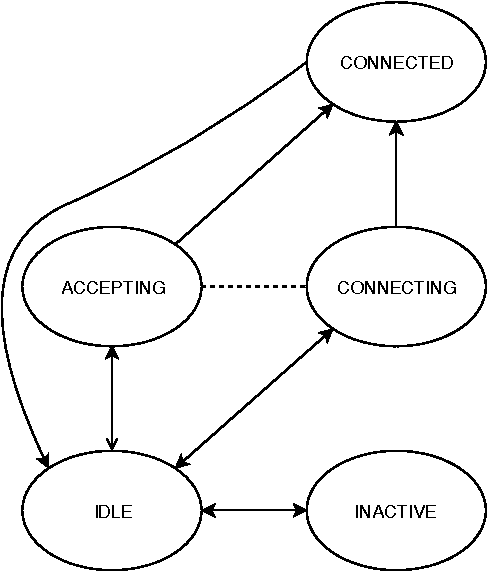
\includegraphics[width=0.5\textwidth]{p2p-State.pdf}
    	   \caption[Zustandsmodell eines p2p Verbindungsaufbaus]{Das Zustandsmodell eines p2p Verbindungsaufbaus zeigt die von außen beobachtbaren Zustände für eine erfolgreiche Nutzung einer p2p Verbindung. } \label{p2p:state}
	\end{figure}   

    Ein besonderer Nutzungspunkt für p2p Verbindungen stellen IoT-Geräte dar, da so zum einen Kommunikation ohne Konfiguration des Nutzers zwischen den IoT-Geräten stattfinden kann und eine Konfiguration der IoT-Geräte durch den Nutzer stattfinden kann ohne Peripherie an das Gerät anschließen zu müssen. Internet of Things ist ein Sammelbegriff für Gebrauchsgegenstände wie Heizungsthermostate oder Maschinen wie CNC-Fräsen, die in einer moderneren Interpretation ihrer Funktionalität über ein Netzwerk untereinander und mit Servern kommunizieren. Anwendungsgebiete können die Hausautomation, Sensornetzwerke und Betriebsüberwachung von Maschinen sein. In einem weiter gefassten Blickfeld wird unter diesem Begriff auch die Vernetzung von ganzen Städten und deren Infrastruktur untersucht \cite{ituGroup}.
    
    \subsection{Services}
    Für solche IoT-Geräte muss eine Erstkonfiguration initial vorgenommen werden, um eine Kommunikation mit anderen Geräte zu ermöglichen. Da nicht jedes Gerät einen Bildschirm oder komplexe Eingabemöglichkeiten besitzt, ist es sinnvoll, diese Einrichtung auf ein Smartphone auszulagern, wie es bereits im vorausgegangenen Projekt geschehen ist. Da die Konfiguration durch einen REST-Server angeboten wird, ist es so auch möglich, weitere Konfigurationsmöglichkeiten für Sensoren und Aktuatoren als weiteren Service anzubieten.
    
    Ein Service definiert sich als ein Dienst, welcher Anderen eine Leistung oder Aufgabe bereitstellt und im Sinne, eine Einheit von Programmen, welcher durch eine Schnittstelle eine Funktionalität verwaltet und bereitstellt. Ein Service kann eine solche Schnittstelle auf verschiedene Arten bereitstellen, jedoch sollten solche Schnittstellen über Verträge abgesichert werden, um ungewollte Änderungen im Betrieb zu vermeiden und eine reibungslose Anbindung von neuen Funktionalitäten zu gewährleisten \cite[S.11]{finger}.
    
    Im Rahmen einer Anwendungsarchitektur als Sammlung von {\it Microservices} treten Services als {\it Messagehandler} auf und definieren ihre Schnittstellen durch Nachrichten oder {\it RPC} Aufrufe. Microservices können dabei wiederum als Services betrachtet werden. Vorteile bietet eine solche Architektur in einer leichten Skalierbarkeit der Anwendung oder einzelner Teile und einer sauberen Kapselung von Anwendungsteilen. Zwischen {\it Messagehandlern} wird oftmals auf Authentifizierung verzichtet, wenn die teilnehmenden Dienste bekannt sind, da auf diese Weise ein höherer Durchsatz erzielt werden kann \cite{microservices}.
    
    Ein {\it Daemon}, welcher eine Hardwarekomponente verwaltet, kann ebenfalls als Service, welcher abstraktere Funktionalität auf dieser Hardware bereitstellt, definiert werden. Auf diese Kategorie von Services trifft die Einschränkung der Einzigartigkeit zu, da immer eine Systemresource nur von einem Programm genutzt werden kann.
    
    Im simpelsten Fall kann ein Service auch als Server definiert werden, um seine Funktionalität Clients zur Verfügung zu stellen. Dies bietet sich besonders dann an, wenn verschiedene Architekturen von Clients in einer hohen Anzahl den selben Service benutzen sollen oder Clients zunächst eine Authentifizierung vornehmen sollen. 
    Ein klassisches Client/Server-Modell sieht hierbei vor, dass auszuführende Berechnungen so aufgeteilt werden, dass ein Server Daten konsistent nutzen kann und in der Lage ist, die verwalteten Daten mehreren Clients auszuliefern. \cite[S.8]{abts}
        
%    \subsection{Servicestabilität (Todo: entfällt eventuell)}
%    - API Versionierung
    
%    - Absichern von Änderungen durch Contract-Driven-Development
    
%    - Integrationstests
    \subsection{Netzwerktopologie}
    
    Der Begriff {\it peer-to-peer} beschreibt eine Art von infrastrukturlosen Netzwerk zwischen zwei oder mehr lokalen Geräten. Um die Vor- und Nachteile einer solchen Verbindung darstellen zu können, werden zunächst die unterschiedlichen Netzwerktypen gegenüber gestellt. Ebenso ist es sinnvoll die zu evaluierenden Technologien in verschieden Topologien einzuordnen, um sie im Hinblick auf Reichweiten und Eigenschaften vergleichen zu können.
    
    {\it Ad Hoc} Netzwerktechnologien erlauben es zwei oder mehr Geräten ein dezentrales Netzwerk aufzubauen. Um die Kontrolle über die gemeinsame Schnittstelle zu erlangen, agiert hierbei entweder eines der Geräte als Verwalter der Verbindung oder es werden spezielle Sequenzen zum Frequenzwechsel in Verbindung mit einer Kollisionsauflösung durch zufällig langes Warten definiert, um Kommunikationskollisionen zwischen Teilnehmern zu vermeiden.
    
    Im Gegensatz zum dezentralisierten {\it ad hoc} Netzwerk nutzt ein Stern-basiertes Netzwerk Knotenpunkte, um die Kommunikation zu Endgeräten zu übernehmen. Wi-Fi bildet ein solches Netzwerk mit {\it Access Points} ab, da diese ein gemeinsames Übertragungsmedium aller verbundenen Endgeräte verwalten und keine Endgeräte direkt miteinander kommunizieren. Ein solches Netzwerk ist dann sinnvoll, wenn der Übergang zu einem anderen Netzwerk in einer Singularität verwaltet werden soll und Endgeräte generell wenig untereinander kommunizieren, da eine Datenübertragung so die doppelte Bandbreite benötigt, um die selbe Übertragungsgeschwindigkeit zu erzielen, da Pakete zunächst zum Knotenpunkt übertragen werden und dieser die Pakete über das gemeinsame Medium erneut an das Zielgerät übermittelt.

    Alle zu überprüfenden Technologien bilden ein {\it ad hoc}, da das Ziel ist, das IoT Gerät erst in ein Wi-Fi Netzwerk zu bringen und somit noch keine gemeinsame Netzwerkverbindung besteht. Relevant ist auch, dass lokale Geräte in einem Raum angesprochen werden können, ohne große Distanzen überbrücken zu müssen. Die genutzten Technologien gehören unterschiedlichen Topologien an, wodurch sich ihre Einsatzgebiete auch unterscheiden:
    \begin{itemize}
    \item {\it Wi-Fi Direct} ist ein Wireless Local Area Network (WLAN) und kann in dieser Kategorie über theoretische Distanzen von bis zu 100 Metern Daten übertragen. Ähnlich zu Wi-Fi ist die Signalstärke von Wi-Fi Direct ausreichend, um in einem Gebäude eine Verbindung zu anderen Geräten aufbauen zu können. Da Signale stark durch Objekte und Wände gedämpft werden, reduziert sich jedoch die Reichweite innerhalb von Gebäuden drastisch wodurch eine Einordnung als Personal Area Network (PAN) zutreffender ist.
    
    \item {\it Bluetooth} ordnet sich ebenfalls als PAN ein und erlaubt den Datenaustausch bis zu einer theoretischen Distanz von 10 Metern. Dies ist ausreichend, um Geräte im Bereich um die eigene Person anzusteuern, was eine durchschnittliche Raumgröße abdeckt. Bluetooth untertützt eine Vielzahl von Protokollen, insbesondere zur Audioübertragung. Typische Anwendungsfälle sind hierbei drahtlose Peripheriegeräte und der lokale Dateienaustausch.
    
    \item {\it NFC} kann lediglich Distanzen von unter 10 Zentimetern überbrücken, und kommt so größtenteils in Verbindung mit mobilen Zahlungsmitteln zum Einsatz. NFC ist zum einen der Name der eingesetzten Technologie als Weiterführung von RFID, gleichzeitig beschreibt es jedoch auch eine Netzwerktopologie, die es Geräten erlaubt auf einem engen Raum miteinander zu kommunizieren. 
    
    \item {\it USB} ist ein kabelgebundenes Übertragungsmedium und erfordert so einen direkten Zugang zum Raspberry Pi. Da in der Spezifikation zu USB 2.0 eine maximale Kabellänge von 5 Metern definiert ist \cite{usbSpec}, ordnet sich dieser Standard ebenfalls als PAN ein.
    
    \end{itemize}
    \section{Grundlagen der Verbindungstechnologien}
	Da die Nutzbarkeit der Übertragungstechnologien für die Verbindungskonfiguration bereits in \cite{aiProject} überprüft wurden, soll noch einmal jede Technologie in ihrer Funktionsweise kurz vorgestellt werden und der Ablauf eines Verbindungsaufbaus beschrieben werden.
	\subsection{Bluetooth}
	
	\subsection{NFC}
	
	\subsection{USB}

    \section{Eigene Umsetzung}
        Im Folgenden wird die Implementierung einer p2p Verbindung über Bluetooth, NFC und USB beschrieben. Jede dieser Technologien soll zunächst separat betrachtet werden, um Details und Probleme bei der Implementierung aufzuzeigen.
        
        Bei der Kapselung von HTTP Anfragen muss bedacht werden, wie eine Technologie Verbindungen zur Verfügung stellt, da so zwischen kurzlebigen Verbindungen ähnlich zu HTTP Anfragen und langlebigen Verbindungen wie einer Datenübertragung per Kabel unterschieden werden muss. Letztere weisen dabei das Problem auf, HTTP Anfragen, die mit einem {\it EOF} beendet werden, über eine langlebige Verbindung zu senden, da ein {\it EOF} immer auch das Ende der Verbindung aufzeigt.
        
    \subsection{HTTP Kapselung}
        Um eine p2p Verbindung unabhängig von der genutzten Verbindungstechnologie nutzen zu können, ist es nötig, eine HTTP Verbindung zum existierenden REST-Server aufbauen zu können. Da das REST-Prinzip eng mit HTTP verbunden ist, sind auch die Implementierungen von REST meistens fest mit einem HTTP Server oder Client verbunden. Auf der Serverseite stellt dies kein Problem dar, da der HTTP-Server nicht von den genutzten Sockets entkoppelt werden muss. Dazu wird ein zweiter Server vorgeschaltet, welcher lokale Sockets nutzt um mit dem eigentlichen Server zu kommunizieren und den Verbindungsaufbau sowie Verbindungsabbau für die genutzte Technologie und deren mögliche virtuelle Socket-Verbindung zu verwalten.
        
        \begin{lstlisting}[frame=bt, label={lst:socket:create}, language=C, caption=Instanziierung eines Sockets (Servercode in C)]
int s = socket(AF_INET, SOCK_STREAM , 0);
struct sockaddr_in rem_addr = { 0 };
rem_addr.sin_addr.s_addr = htonl(INADDR_LOOPBACK);
rem_addr.sin_family = AF_INET;
rem_addr.sin_port = htons(targetPort);
connect(s, (struct sockaddr *)&rem_addr , sizeof(rem_addr));
        \end{lstlisting}
        Wie im \reflst{lst:socket:create} zu sehen, baut der kapselnde Server eine Socket-Verbindung auf, um Daten zum Zielserver zu senden. Diese Verbindung wird erst aufgebaut, sobald das Endnutzergerät kurz davor steht eine Anfrage an den Zielserver zu stellen, um mögliche Zeitüberschreitungen im HTTP-Server zu vermeiden. Dies erfüllt sonst die Anfangskriterien eines slow-louis-Angriffes auf einer einzelnen Verbindung. \footnote{Quelle?}
        \begin{lstlisting}[frame=bt, label={lst:socket:data}, language=C, caption=Datenweiterleitung durch Sockets (Servercode in C)] 
int pipeData(int sourceSocket, int sinkSocket, char* buffer) {
    int bytes_read = read(sourceSocket, buffer, BUF_SIZE);
    if(bytes_read < 0) return -1;
    if(bytes_read == 0) return -20; // indicates an EOF
    int bytes_sent = send(sinkSocket, buffer, bytes_read, 0);
    if(bytes_sent < 0) return -2;
    return 0;
}
        \end{lstlisting}
        
        Die bestehende Socket-Verbindung zum Zielserver wird genutzt, um die ankommenden Daten und deren Antworten voll duplex weiterzuleiten. Dies ist realisiert, indem eine Methode {\it pipeData} in zwei Threads mit invertiertnm {\it sourceSocket} und {\it sinkSocket} aufgerufen wird, bis ein {\it EOF} gesendet wird (\reflst{lst:socket:data}). Für den kapselnden Server ist es so unerheblich, welche Seite Daten zuerst senden möchte. Die Verbindung zwischen dem Zielserver und dem kapselnden Server kann so auch unabhängig von der Verbindung zum Endgerät verwaltet werden, da beim Lesen der Daten vom Zielserver ein{\it EOF} das Ende der Verbindung zum Zielserver aufzeigt. Die Verbindung zum Endgerät muss so nicht zwingend geschlossen werden.
        
        Ein Abkapseln der Technologie über einen weiteren Server auch auf Seite des Clients erscheint als vermeidbarer Overhead, da so keine Serverimplementierung auch im Client stattfinden muss. Stattdessen wird hier der HTTP-Client, welcher der REST-Bibliothek zugrunde liegt, so aufgetrennt, dass keine TCP/IP-Verbindungen aufgebaut werden, jedoch die Anfragen aus der Bibliothek als String entnommen werden können und  deren Antworten als String eingespeist werden können. Für den REST-Client retrofit wird intern okhttp\footnote{Referenz} als HTTP-Client genutzt. Um zu verstehen, welche Änderungen am Client nötig sind, sollte zuerst die interne Struktur der okhttp Bibliothek erläutert werden.
        \begin{lstlisting}[frame=bt, label={lst:android:okhttp}, language=Java, caption=Interner Aufbau von okhttp (Clientcode in Java)]
List<Interceptor> interceptors = new ArrayList<>();
...
interceptors.add(retryAndFollowUpInterceptor);
interceptors.add(new BridgeInterceptor(client.cookieJar()));
interceptors.add(new CacheInterceptor(client.internalCache()));
interceptors.add(new ConnectInterceptor(client));
...
interceptors.add(new CallServerInterceptor(forWebSocket));
        \end{lstlisting}
        Serveraufrufe werden im okhttp Client (\reflst{lst:android:okhttp})\footnote{\cite{okhttpRealCall} Zeilen 185-194)} durch eine Kette von Interceptors verarbeitet. Jeder {\it Interceptor} hat dabei die Möglichkeit den Aufruf oder die Kette beliebig zu verändern und in dieser Liste nimmt jeder Interceptor eine andere Rolle ein. Der {\it RetryAndFollowUpInterceptor} stellt in der Kette eine {\it StreamAllocation} bereit und übernimmt das Abbrechen von Aufrufen. Der darauf folgende {\it BridgeInterceptor} verwaltet Cookies aus den Anfragen und Antworten, sowie die Übersetzung von Anwendungsanfragen zu Netzwerkanfragen. Dies beinhaltet ebenfalls die Verwaltung von netzwerkrelevanten Headern wie zum Beispiel den "User-Agent"-Header oder "Content-Encoding"-Header. Wie der Name des {\it CacheInterceptor} bereits vermuten lässt, wird in diesem das Speichern und Abrufen von Antworten auf wiederkehrende Anfragen ermöglicht. Sowohl Cookies als auch der Cache lassen sich einfach umgehen, indem der Client jeweils kein Objekt ausliefert oder ein Objekt bereitstellt, welche alle Methoden mit leeren Ergebnissen quittiert. Bevor der Aufruf vom {\it CallServerInterceptor} tatsächlich ausgeführt wird und auf ein Ergebnis gewartet wird, Baut der {\it ConnectInterceptor} noch eine HTTP-Verbindung über die {\it StreamAllocation} der Kette auf. Für diese Verbindung wird dann ein {\it HTTPCodec} genutzt, um die Anfrage auf den Socket zu schreiben und die Antwort zu lesen.
        
        \begin{lstlisting}[frame=bt, label={lst:android:okhttpchanges}, language=Java, caption=Änderungen an okhttp (Clientcode in Kotlin)]
val interceptors = ArrayList<Interceptor>()
...
interceptors.add(BridgeInterceptor(wrapper.cookieJar()))
interceptors.add(CacheInterceptor(wrapper.internalCache()))
...
interceptors.add(SimpleServerInterceptor(wrapper.httpCodec()))
        \end{lstlisting}
        \footnote{Todo: Rahmen um Code} Im Gegensatz zur okhttp Implementierung muss die p2p Verbindung so verwaltet werden, wie es von der Implementierung der Technologie vorgegeben wird. Dazu wird der {\it RetryAndFollowUpInterceptor} sowie der {\it ConnectInterceptor} weggelassen und der {\it CallServerInterceptor} im {\it SimpleServerInterceptor} soweit vereinfacht wird, sodass dieser keine Handshakes mehr unterstützt und nicht mit Websockets genutzt werden kann.
        Um die Kapselung so simpel wie möglich zu halten, wird ebenfalls auf HTTP 2 verzichtet, wodurch der abgewandelte HTTP Client nur HTTP1.1 unterstützt. Da im okhttp Client der {\it HttpCodec} sowohl die Aufgabe erfüllt, den Request in einen HTTP-String umzuwandeln, als auch den Request über die Verbindung zu schreiben, muss so lediglich eine weitere Klasse angepasst werden. der {\it Http1Codec} wird dabei minimal angepasst, sodass interne Klassen der okhttp Implementierung, die nicht im Rahmen dieser HTTP Kapselung nötig sind, genutzt werden.
        
        
        Diese generische HTTP Kapselung lässt sich nun ähnlich der okhttp Implementierung über eine zentrale Klasse, den {\it SimpleHttpWrapper} nutzen. Diese Klasse nutzt ebenfalls das Builder-Pattern, um so nah wie möglich an der okhttp Bilbiothek zu bleiben. Über diesen Builder lässt sich nun ein {\it ConnectionStream} definieren, welcher dann den Inputstream und Outputstream der Verbindung bereitstellt.
        
        \subsection{Bluetooth}
        Die Umsetzung einer p2p Verbindung über Bluetooth besteht darin, dass ähnlich zu HTTP Sockets, RFCOMM Sockets genutzt werden, um mit einem Server kurzweilig zu kommunizieren. Jede dieser RFCOMM Verbindungen bildet hierbei eine HTTP Anfrage und HTTP Antwort ab. Wie bereits in der HTTP Kapselung beschrieben, wird die Verbindung von selbst wieder geschlossen, sobald ein EOF gesendet wird. Da RFCOMM Socket Verbindungen ein automatisches Pairing mit Schlüsselaustausch durchführen, ist keinerlei Eingriff oder Bestätigung des Nutzers nötig, um Daten übertragen zu können.
        \begin{lstlisting}[frame=bt, label={lst:android:bluetooth}, language=Java, caption=Verbindungsaufbau mit Bluetooth (Clientcode in Kotlin)]
val bluetoothDevice = bluetoothAdapter.bondedDevices?.firstOrNull { bluetoothDevice ->
    bluetoothDevice.address == device.bluetoothDetails.mac
} ?: bluetoothAdapter.getRemoteDevice(device.bluetoothDetails.mac)

val method = bluetoothDevice::class.java.getMethod("createInsecureRfcommSocket", Int::class.javaPrimitiveType)
val socket = method.invoke(bluetoothDevice, device.bluetoothDetails.port) as BluetoothSocket
socket.connect()
        \end{lstlisting}
        Für den Verbindungsaufbau muss die Bluetooth MAC-Addresse sowie der Bluetooth Port angegeben werden. Der {\it BluetoothAdapter} aus dem Android Framework gibt ein {\it BluetoothDevice} für die angegebene MAC-Addresse zurück. Es ist hierbei noch unerheblich, dass dieses Gerät auch in der Nähe erreichbar ist oder existiert. Über die versteckten Methoden {\it BluetoothDevice::createInsecureRfcommSocket} und {\it BluetoothDevice::createRfcommSocket} kann eine Socket-Verbindung zu einem bestimmten Port des entfernten Gerätes erstellt werden. In Android sind diese Methoden versteckt, um Konflikte zwischen Apps beim festlegen der Portnummern zu vermeiden, da lediglich 30 RFCOMM Ports zur Verfügung stehen.\footnote{Quelle z.B. https://people.csail.mit.edu/albert/bluez-intro/x148.html} Stattdessen sollen Services eine UUID generieren, welche über Bluetooth Service Discovery Protocol (SDP) von anderen Geräten abgefragt werden kann. Das SDP Protokoll übernimmt dann die Vergabe von Ports für die registrierten Services. Um diese exemplarische Implementierung jedoch simpel zu halten und volle Kontrolle über das Servergerät besteht, wird hierbei ein vordefinierter Port genutzt.

         Jegliche Logik zum tatsächlichen Verbindungsaufbau ist in der Methode {\it BluetoothSocket::connect} gekapselt und muss bei der Umsetzung nicht beachtet werden. Auf beiden Geräten muss lediglich Bluetooth eingeschaltet sein und das Servergerät muss auffindbar für den Client sein.
   
        \begin{lstlisting}[frame=bt, label={lst:bluetooth:socket}, language=C, caption=Verbindungsaufbau mit Bluetooth (Servercode in C)]
int s = socket(AF_BLUETOOTH, SOCK_STREAM, BTPROTO_RFCOMM);
struct sockaddr_rc loc_addr = { 0 };
loc_addr.rc_family = AF_BLUETOOTH;
loc_addr.rc_bdaddr = *BDADDR_ANY;
loc_addr.rc_channel = (uint8_t) bluetoothPort;
bind(s, (struct sockaddr *)&loc_addr, sizeof(loc_addr));
listen(s, LISTEN_QUEUE_SIZE);
        \end{lstlisting}
        Auf Seite des Servers kann die Implementierung der HTTP Kapselung fast vollständig übernommen werden,jedoch müssen Verbindungen auf einem weiteren Socket mit dem Bluetooth RFCOMM Protokoll akzeptiert werden.
        
        Mit diesen beiden Anbindungen von Bluetooth an die generische HTTP Kapselung lässt sich diese simple Lösung bereits nutzen. Um jedoch die geheimen Methoden unter Android nicht nutzen zu müssen, ist es nötig, auf dem Server die Anbindung im Bluetooth SDP als Service zu hinterlegen. Kürzlich wurde die BlueZ 5 Bibliothek von einer simplen C-Schnittstelle auf eine DBus-Schnittstelle umgewandelt.\footnote{\cite{BluezMigration}} Dies hat zur Folge, dass viele der Beispiele und Erklärungen, ebenso wie Bücher nicht mehr aktuell sind und erst auf die neue API hingewiesen wird, wenn nach der expliziten Fehlermeldung gesucht wird.
        
        \begin{lstlisting}[frame=bt, label={lst:bluetooth:sdp}, language=C, caption=Veraltete Nutzung von SDP (Servercode in C)]
sdp_set_info_attr(record, serviceName, serviceProvider, serviceDescription);
*session = sdp_connect(BDADDR_ANY, BDADDR_LOCAL, SDP_RETRY_IF_BUSY);
sdp_record_register(*session, record, 0);
        \end{lstlisting}
        In älteren Versionen von BlueZ war es möglich einen SDP Eintrag mit der Methode {\it sdp\_record\_register} anzulegen. Dieser Eintrag wurde von SDP selbstständig verwaltet und entfernt wenn die Sitzung zu SDP beendet wurde. Auf Grund des Wechsels zu DBus kann diese SDP-Schnittstelle nicht mehr genutzt werden, da sich keine Sitzungen zum SDP daemon aufbauen lassen, da dieser nicht mehr existiert.
        \begin{lstlisting}[frame=bt, label={lst:bluetooth:dbus}, language=C, caption=DBus Nutzung von SDP (Servercode in C)]
static DBusHandlerResult wrapper_messages(DBusConnection* connection, DBusMessage* message, void* user_data) {
    const char* interface_name = dbus_message_get_interface(message);
    const char* member_name = dbus_message_get_member(message);
    if (0==strcmp("org.bluez.Profile1", interface_name)) {
        if(0==strcmp("Release", member_name)) {
            profileRelease();
            return DBUS_HANDLER_RESULT_HANDLED;
        } else if(0==strcmp("NewConnection", member_name)) {
            profileNewConnection(message);
            return DBUS_HANDLER_RESULT_HANDLED;
        } else if(0==strcmp("RequestDisconnection", member_name)) {
            profileRequestDisconnection();
            return DBUS_HANDLER_RESULT_HANDLED;
        }
    }
    return DBUS_HANDLER_RESULT_NOT_YET_HANDLED;
}

DBusObjectPathVTable vtable;
vtable.message_function = wrapper_messages;
vtable.unregister_function = NULL;              

DBusConnection* conn = dbus_bus_get(DBUS_BUS_SYSTEM, &err);
dbus_connection_try_register_object_path(conn, PROFILE_PATH, &vtable, NULL, &err);

DBusMessage* msg = dbus_message_new_method_call("org.bluez", "/org/bluez", "org.bluez.ProfileManager1", "RegisterProfile");
...
dbus_connection_send_with_reply_and_block(conn, msg, -1, &err);
        \end{lstlisting}\footnote{TODO: Code Beispiel ist zu lang.}
        Um die SDP Funktionalität dennoch nutzen zu können, wird im \reflst{lst:bluetooth:dbus} gezeigt, wie ein Callback-Objekt registriert wird. Dieses Objekt hat die Aufgabe, ankommende Verbindungen zu akzeptieren und zu nutzen. Es ersetzt somit den akzeptierenden Serversocket. Weiterhin muss das Objekt in der Lage sein, bestehende Verbindungen schließen zu können. Dies hat zur Folge, dass die Komplexität im Vergleich zu einer Lösung ohne SDP stark erhöht wird, da nicht nur die DBus Nachrichten auf einem separaten Thread gehandhabt werden müssen, sondern auch eine Auflösung zwischen offenen Dateideskriptoren und den Client Kennungen stattfinden muss.
        Über diese gegebenen Dateideskriptoren konnte jedoch keine erfolgreiche Datenübertragung erzielt werden. Eine Verbindung wurde immer erfolgreich aufgebaut, jedoch schienen keine Daten tatsächlich übertragen zu werden, wodurch die Verbindung nach einem Timeout wieder geschlossen wurde.
        
        Ebenso war es serverseitig nicht möglich, die nötigen Sockets in pharo zu verwalten. Dem liegt zu Grunde, dass Sockets in der pharo VM über das SocketsPlugin\footnote{Quelle: https://github.com/pharo-project/pharo-vm/tree/master/mc/VMMaker.oscog.package/SocketPlugin.class} gekapselt verwaltet werden und dort fest als IP-Sockets erstellt werden.
        \begin{lstlisting}
newSocket = socket(AF_BLUETOOTH, SOCK_STREAM, BTPROTO_RFCOMM);

        \end{lstlisting}
    \subsection{NFC}
		
    \subsection{USB}

    \section{Ergebnisse der Evaluation}
		Durch die Betrachtung der Umsetzungsmöglichkeiten der einzelnen p2p Technologien kann nun eine Evaluation auf Grundlage der definierten Ziele vorgenommen werden. Zum Vergleich wird Wi-Fi Direct als bereits implementierte Technologie genutzt, um einen Bezug zur bestehenden Lösung aufbauen zu können.
		\subsection{Zuverlässigkeit}
		Die Robustheit der einzelnen Technologien bei Fehlern und die Reproduzierbarkeit von Verbindungen bilden zusammen das Kriterium der Zuverlässigkeit. Wie bei Wi-Fi Direct bereits deutlich wurde, sind diese beiden Punkte nicht zwingend für jede Technologie ausreichend gegeben.
		
		\begin{itemize}
		\item {\it Wi-Fi Direct:} Eine hohe Fehleranfälligkeit in Kombination mit einer schlechten Fehlererholung durch Abstürze des laufenden Wi-Fi Daemon führen zu einer unzureichenden Zuverlässigkeit von Wi-Fi Direct. Ebenso konnte beobachtet werden, dass die internen Zustände der genutzten Bibliothek weder dokumentiert sind, noch waren diese Zustände sauber voneinander gekapselt, wodurch der Erfolg eines Verbindungsaufbaus von vorhergehenden Verbindungen abhängt. Die internen Zustandswechsel konnten zwar über Events der Bibliothek beobachtet werden, jedoch wurden daraus die Menge der möglichen Zustände und deren Übergänge nicht deutlich, da nicht zwingend jedes Event einem neuen Zustand entspricht. Die Dokumentation des {\it wpa\_supplicant} versäumt es ebenfalls zu beschreiben, in welcher Reihenfolge ein erfolgreicher Verbindungsaufbau vollzogen wird, wodurch nicht sichergestellt werden kann, dass die eigene Anbindung der erwarteten Nutzung entspricht.
		Zwar steht der Sourcecode der {\it wpa\_supplicant} Bibliothek und damit auch die Schnittstelle als Sourcecode zur Verfügung, da jedoch die Schnittstelle über Nachrichten statt über Methoden genutzt wird, ist es schwierig zu erkennen, welche Teile des Sourcecodes relevant sind. Es kommt hierbei erschwerend hinzu, dass nicht jede Bibliothek mit den gleichen Parametern gebaut wird, wodurch nicht zwingend der volle Funktionsumfang zur Verfügung steht.
		
		\item {\it Bluetooth:} Im Gegensatz dazu konnte mit Bluetooth und der genutzten Bibliothek ein Verbindungsaufbau mit reproduzierbaren Ergebnissen erreicht werden. Durch das integrierte Hilfsmittel {\it bluetoothctl} der BlueZ Bibliothek kann die Menge der bestehenden Zustände gut beobachtet werden. Die Benennung der einzelnen Zustände orientiert sich hierbei an der theoretischen Spezifikation von Bluetooth, wodurch auch die Zustandsübergänge bereits klar werden. Eine feinere Betrachtung der Zustände ist nicht nötig, da die Bluetooth Bibliothek jeglichen Zustand der Verbindung selbstständig verwaltet und dies der Anwendung als Serversocket zur Verfügung stellt. Fehler werden somit als Schließen des Sockets oder Fehler des Verbindungsaufbaus bekannt gemacht. Daraus lässt sich nicht der exakte Grund Ableiten lässt, jedoch besitzt Bluetooth aufgrund des saubere definierten Zustandsmodells und durch Socketverbindungen auch die Anbindung von Bluetooth eine solche Fehlerstabilität, dass die Verbindung lediglich neu aufgebaut werden muss \cite{bluetoothSpec}.
		
     \item {\it NFC:} Wenn ein bereits bestehender Wrapper genutzt wird, besteht das Problem, dass nicht ersichtlich ist, wann Fehler auftreten können. Die Kapselung auf Socketverbindungen für NFC ermöglicht es jedoch auch, eine Behandlung von Fehlern durch das Schließen bestehender Verbindungen durchzuführen und eine Verbindung erneut aufzubauen. Die internen Zustände eines NFC Verbindungsaufbaus lassen sich nicht direkt über die genutzte Bibliothek {\it libnfc} beobachten, jedoch kann über das Hilfsmittel {\it nfc-poll} ein NFC Gerät und die ausgetauschten Befehle ausgelesen werden. Eine Reproduzierbarkeit von Verbindungen ist durch das von NFC genutzte Trägersignal zwar gegeben, jedoch wird in der genutzten Implementierung ein hochfrequentes {\it Keep-Alive} Signal genutzt, damit die Verbindung aufrecht erhalten wird.
     
     \item {\it USB:} Ähnlich zu NFC schränkt die bestehende Implementierung von USB das Fehlerverhalten der zugrundeliegenden {\it libusb} Bibliothek ein und bündelt dieses ebenfalls über eine Socketverbindung. Da der Verbindungsaufbau von USB Geräten bereits vom Kernel übernommen wird, können Zustandsübergänge an neuen Geräten über {\it udev} beobachtet werden. Eine Fehleranfälligkeit der USB Verbindung ergibt sich aus den genutzten Treibern. Da jedoch das USB-Gerät ohne Treiber mit {\it libusb} angesprochen wird, besteht eine sehr geringe Fehleranfälligkeit einer USB Verbindung, da diese kabelgebunden ist und sich erst eine Fehleranfälligkeit aus den genutzten Treibern oder einer Abweichung von der USB Spezifikation ergibt \cite{usbSpec}. Die Spezifikation sieht eine Fehlererholung so vor, dass der Host der Verbindung laufende Datentransfers steuern kann. Diese Fehler werden erst propagiert, wenn sie nicht erfolgreich abgefangen werden konnten. Diese Fehler tauchen dann lediglich im Log des Kernels auf und resultieren in einem Zurücksetzen der USB Verbindung über das Hotplugging von USB.
		\end{itemize}
		
		\subsection{Wartbarkeit}
		Fehler in der Nutzung einer Technologie lassen sich nur dann leicht beheben, wenn die Dokumentation so vollständig ist, dass sie den betroffenen Nutzungsfall abdeckt und somit eine Abweichung der Anbindung von der Dokumentation aufgedeckt werden kann. Sollte die Dokumentation jedoch nicht ausreichend auf diesen Fall eingehen, muss der Quellcode der angebotenen Schnittstelle zur Verfügung stehen und leicht zu verstehen sein, sodass die Abweichung leicht gefunden werden kann. Sollten Tests für die genutzten Bibliotheken im Sourcecode vorhanden sein, verbessert dies die externe Wartbarkeit ebenfalls, da so zum Einen bereits eine Abstraktion der Hardware besteht und diese für eigene Tests genutzt werden kann und zum Anderen die Nutzung der Bibliothek anhand der getesteten Nutzungsfälle exemplarisch gezeigt wird.
		
		\begin{itemize}
		\item {\it Wi-Fi Direct:} Die Dokumentation von Wi-Fi Direct ist bei der Wi-Fi Association nicht öffentlich zugänglich, jedoch enthält die Beschreibung der {\it wpa\_supplicant} Implementierung eine Aufstellung einiger Ereignisse, die bei der Nutzung auftreten können. Fehler beim Verbindungsaufbau oder während der Verbindungsnutzung werden zwar als solche Ereignisse der Anbindung mitgeteilt, jedoch ließen sich auch eine mangelnde Fehlerrobustheit durch Abstürze bei einigen dieser Ereignisse feststellen. Tests sind im {\it wpa\_supplicant} für die einzelnen Schritte eines p2p Verbindungsaufbaus als Python-Skripte vorhanden und basieren auf einer simulierten Hardware. Diese simulierte Hardware lässt sich somit auch für eigene Tests nutzen, um die eigene Implementierung mit möglichst geringen Abänderungen testen zu können.
		
		\item {\it Bluetooth:} Eine Anbindung an Bluetooth geschieht über Sockets, welche bei der Erstellung durch das Austauschen einiger Parameter bereits eine testbare Umgebung bereitstellen können. Weiterhin wird die Spezifikation von Bluetooth durch die Bluetooth SIG öffentlich einsehbar bereitgestellt und beschreibt ausführlich interne Zustände einer Bluetooth Implementierung sowie die Testbarkeit eines Bluetoothgerätes\cite{bluetoothSpec}. Die BlueZ Bibliothek steht ebenfalls als Referenz zur Verfügung und enthält in den Tests ebenfalls eine Beispielanbindung für die Nutzungsfälle der Bibliothek jedoch keine Virtualisierung der Hardware. Dies bedeutet, dass für einen vollständigen Integrationstest mindestens zwei Bluetoothschnittstellen am testenden Gerät vorhanden sein müssen, da ein Loopback ebenfalls nicht möglich ist.
		
		\item {\it NFC:} Die existierende Lösung nutzt ebenfalls Sockets um eine Kommunikation aufbauen zu können, somit kann auch hier die eigene Implementierung getestet werden, indem dieser Serversocket angesprochen wird. Um auch die Kapselung der NFC Bibliothek testen zu können, ist es nötig, die zugrundeliegende Bibliothek {\it libnfc} zu betrachten. In ihr finden sich sowohl Beispiele für alle unterstützten Nutzungsfälle des genutzten NFC Chips als auch Tests der Bibliothek. Eine Dokumentation der Bibliothek als solche existiert nur minimal, jedoch können die Beispiele genutzt werden eine Implementierung vorzunehmen. Eine Konfiguration von Geräten, die mit der Bibliothek genutzt werden sollen, ist nötig, da die NFC Bibliothek UART zur Kommunikation nutzt und Geräte somit nicht automatisch als NFC-Modul erkannt werden. Ein solcher Konfigurationsaufwand verschlechtert auch die Wartbarkeit der Anbindung, da diese Anbindung nicht ohne die Konfiguration funktionieren kann und sich nicht testen lässt ob eine Konfiguration für alle Anwendungsfälle korrekt ist oder nur für einen getesteten Anwendungsfall richtiges Verhalten zeigt, da eine Dokumentation über die Konfigurationsmöglichkeiten nicht gegeben ist. 
		
     \item {\it USB:} Eine Spezifikation über USB kann öffentlich eingesehen werden, jedoch umschließt diese nicht nur die Definition eines Übertragungsprotokolls sondern auch die vollständige Definition der Hardwareschnittstelle, wodurch die für das Protkoll relevanten Teile schwer auffindbar sind und die Spezifikation dadurch einen geringeren Nutzen im Vergleich zu den anderen Technologien aufweist \cite{usbSpec}. Socketverbindungen werden auch hierbei von der genutzten Implementierung für die Dauer der USB Verbindung aufgebaut und im nicht erholbaren Fehlerfall geschlossen. Intern werden Daten über explizit blockierende Methoden gesendet und empfangen, welche auch Fehler der Verbindung als Resultat ausliefern. Jeder dieser Fehler ist in der Dokumentation der {\it libusb} dokumentiert und gibt Aufschluss darüber, wodurch dieser Fehler aufgetreten ist. Die Bibliothek kann ebenfalls im Quellcode eingesehen werden und enthält Beispiele sowie Tests.
     Einige Beispiel werden ebenfalls gleichzeitig als Tests genutzt, jedoch ist zu beobachten, dass nur sehr grundlegende Tests der Bibliothek durchgeführt werden und keine Tests existieren, die eine vollständige Datenübertragung über ein virtuelles USB Gerät überprüfen. Da das AOA Protokoll implementiert wird, ist es auch nicht möglich, einen Test ohne ein Android Gerät zu vollziehen, da nicht geprüft werden kann, dass die im Protokoll gesendeten Daten auch im vorgesehenen Format gesendet wurden. Testbarkeit und damit auch Wartbarkeit ist somit nur bedingt für eine USB Schnittstelle gegeben.
		\end{itemize}
		
		\subsection{Funktionalität}

      \begin{itemize}
		\item {\it Wi-Fi Direct:}
		\item {\it Bluetooth:}
		\item {\it NFC:}
     \item {\it USB:}
		\end{itemize}
		
		\subsection{Effizienz}

      \begin{itemize}
		\item {\it Wi-Fi Direct:}
		\item {\it Bluetooth:}
		\item {\it NFC:}
     \item {\it USB:}
		\end{itemize}
		
		\subsection{Bedienbarkeit}

      \begin{itemize}
		\item {\it Wi-Fi Direct:}
		\item {\it Bluetooth:}
		\item {\it NFC:}
     \item {\it USB:}
		\end{itemize}
		
		\subsection{Zusammenfassung}
%    \begin{figure}[ht]
%    \centering
%    \begin{tikzpicture}
%        \tkzKiviatDiagram[scale=1.0,label distance=.25cm, radial = 5, gap = 1, lattice = 5]{Zuverlässigkeit,Wartbarkeit,Funktionalität,Effizienz,Bedienbarkeit}
%        %Wi-Fi Direct:
%        \tkzKiviatLine[thick,color=red,mark=none, fill=red!20,opacity=.5](2,2,4,4,3)
%        %Bluetooth:
%        \tkzKiviatLine[thick,color=blue, fill=blue!20,opacity=.5](4,4,4,2,4)
%        %NFC:
%        \tkzKiviatLine[thick,color=yellow, fill=red!20,opacity=.5](4,3,3,1,2)
%        %USB:
%        \tkzKiviatLine[thick,color=green, fill=green!20,opacity=.5](1,3,3,3,1)
%    \end{tikzpicture}
%    \caption{M1} \label{fig:rating}
%    \end{figure}
    \section{Fazit}

Die Überprüfung von Softwarequalität auf einer Kombination aus Technologie und Software stellt die Herausforderung, bewertbare Ergebnisse zu erhalten. Da die Qualitätsmerkmale der Zuverlässigkeit, Wartbarkeit, Funktionalität und Bedienbarkeit lediglich auf Grund von Erfahrungswerten bewertet wurden und ihre Spezifikation wesentlich zu komplex sind, um sie im Rahmen dieser Arbeit vollständig auszuwerten, kann nur eine informale Aussage über die eingesetzten Technologien getroffen werden. Jede der Technologien setzt unterschiedliche Schwerpunkte bei den überprüften Qualitätskriterien, wodurch jede der Technologien für manche Anwendungsfälle in Frage kommt. Der Anwendungsfall einer Verbindungskonfiguration als Client-/Server-Lösung zeichnet sich durch ein geringes Datenvolumen in Verbindung mit teilweise hohen Antwortzeiten auf Anwendungsebene aus. Auf Grund dieser Gegebenheiten wird der Evaluationspunkt der Effizienz übergangen und lediglich anhand der verbleibenden Evaluationspunkte ein Ergebnis der Evaluation gezogen.

Für jede der genutzten Technologien kommt ein HTTP Wrapper zum Einsatz, welcher es ermöglicht, die HTTP Befehle über eine andere Technologie als Wi-Fi zum Server zu übertragen. Dieser Wrapper ist eine simple Lösung, die jegliche Technologie als Sockets abbildet, um eine simple Auswechselbarkeit der Technologien zu ermöglichen. Dies hilft ebenfalls das gesetzte Ziel einer Alternative zu Wi-Fi Direct zu erfüllen, da sich die unterschiedlichen Technologien mit geringem Aufwand parallel in der Anwendung nutzen lassen und so dem Nutzer auch eine Wahl zwischen mehreren Verbindungsarten gelassen werden kann. Ebenso müssen keine Änderungen an den Anbindungen der Technologien vorgenommen werden, wenn die Schnittstelle zur Verbindungskonfiguration erweitert werden soll. Da alle Anbindungen von Technologien die selbe Grundlage nutzen, um sie im Wrapper nutzen zu können, entsteht kein zusätzlicher Wartungsaufwand der existierenden Anbindungen, wenn eine neue Technologie ebenfalls genutzt werden soll.

Während Umsetzung wurde deutlich, dass nicht nur Wi-Fi Direct \linebreak Unzulänglichkeiten in seiner Implementierung besitzt. Alle getesteten Technologien weisen in unterschiedlichen Punkten Probleme auf, die jedoch nicht zwingend die Nutzbarkeit für eine Verbindungskonfiguration beeinträchtigen. Die aufgetretenen Probleme verdeutlichen jedoch noch einmal die unterschiedlichen Ansätze der Technologien.

Bluetooth mangelt es auf Grund des Wechsels der Art von Bibliotheks-API an Dokumentation und allgemeinen Beispielen über die Nutzung der Bibliothek. Gleichzeitig traten Probleme bei der Nutzung von {\it SDP} auf, wodurch eine vereinfachte Lösung über einen expliziten RFCOMM Port genutzt werden muss. Dies hat jedoch den Vorteil, dass die Anbindung von Bluetooth wesentlich simpler ist, da keine DBus-API angesprochen werden muss.

Für eine Nutzung von NFC zeigt sich eine Unzulänglichkeit im Bereich der Benutzbarkeit, da der Nutzer gezwungen ist, das Gerät mehrmals in die direkte Nähe des zu konfigurierenden Gerätes bringen, was je nach Einsatzort keine akzeptable Lösung darstellt. Ebenso basiert NFC auf dem Austausch von kurzen Nachrichten über ein Trägersignal und unterstützt so lediglich eine indirekte Kommunikation  beider Teilnehmer durch das Reagieren auf Befehle, was die Funktionalität der Lösung ein wenig dämpft, da so eine bidirektionale Kommunikation zusätzliche Komplexität birgt.

Eine Verwendung von USB scheitert zur Zeit daran, dass eine AOA Verbindung nicht korrekt aufgebaut werden kann dem kann zu Grunde liegen, dass AOA seit dem Jahr 2012 von Google nicht mehr aktiv weiter entwickelt wurde und inzwischen Fehler in der Anbindung dieses Protokolls existieren. Andererseits ist es auch möglich, dass zusätzlicher undokumentierter Konfigurationsaufwand unter Android vorgenommen werden muss. Da keine erfolgreiche Datenübertragung über USB vollzogen werden konnte, kann diese Technologie auch nicht im Rahmen einer Verbindungskonfiguration genutzt werden.

NFC ist gegenüber USB und Wi-Fi Direct ebenfalls eine bessere Alternative, um p2p Verbindungen zu ermöglichen. Zwar liegen die Bedienbarkeit und Funktionalität nicht auf dem Niveau von Bluetooth, da NFC eine für den Nutzer und die Implementierung umständlichere Technologie nutzt, jedoch werden diese wieder durch die Wartbarkeit und Zuverlässigkeit des Mediums aufgewogen.

In der Evaluation hat sich so Bluetooth als beste Technologie für eine p2p Verbindung durchgesetzt, weil sie die für eine Verbindungskonfiguration relevanten Kriterien den anderen Technologien gegenüber besser erfüllt. Besonders die Bedienbarkeit durch den Nutzer zusammen mit einer sehr guten Wartbarkeit geben Bluetooth einen großen Vorteil gegenüber den verbleibenden Übertragungsmedien. Die Bedienbarkeit stellt das wichtigste Kriterium  der geprüften Softwarequalität dar, da die anderen Merkmal nicht zwingend vom Nutzer wahrgenommen werden und eine Software ohne Nutzer auch keinen Nutzen besitzt.

\subsection{Ausblick?}


    \addcontentsline{toc}{section}{\lstlistlistingname}
    \lstlistoflistings
    \pagebreak
    
    \addcontentsline{toc}{section}{Literaturverzeichnis}
    \renewcommand\refname{Literaturverzeichnis}
    \begin{thebibliography}{10}
        \bibitem[Aneja et al.]{Aneja}Nagender Aneja und Sapna Gambhir: "Profile-Based Ad Hoc Social Networking Using Wi-Fi Direct on the Top of Android" {\it Mobile Information Systems, Volume 2018, Article ID 9469536, 7 pages} (2018).
        \bibitem[Eberhardt et al.]{Kelm} Udo Eberhardt und Hans Joachim Kelm [Hrsg.]: {\it USB - Universal Serial Bus} Franzis, Poing (1999).
        \bibitem[Esnaashari et al.]{Esnaashari} Shadi Esnaashari, Ian Welch und Peter Komisarczuk: {\it Determining home users' vulnerability to Universal Plug and Play (UPnP) attacks} Erschienen in: Proceedings of the 2013 27th International Conference on Advanced Information Networking and Applications Workshops (WAINA). IEEE, 2013. - S. 725-729. - ISBN 9781467362399 .
        \bibitem[Kaiser et al.]{Kaiser} Daniel Kaiser, Marcel Waldvogel, Holger Strittmatter und Oliver Haese: {\it User-Friendly, Versatile, and Efficient Multi-Link DNS Service Discovery} Erschienen in: Proceedings 2016 IEEE 36th International Conference on Distributed Computing Systems Workshops : ICDCSW 2016. - Piscataway, NJ : IEEE, 2016. - S. 146-155. - ISBN 978-1-5090-3686-8.
        \bibitem[Kaiser, Waldvogel]{Kaiser2} Daniel Kaiser und Marcel Waldvogel: {\it Adding Orivacy to Multicast DNS Service Discovery} Erschienen in: Proceedings - 2014 IEEE 13th International Conference on Trust, Security and Privacy in Computing and Communications (TrustCom) ; Beijing, China, 24 Sep - 26 Sep 2014. - Piscataway : IEEE, 2014. - S. 809-816. - ISBN 978-1-4799-6513-7.
        \bibitem[Langer et al.]{Langer}Josef Langer und Michael Roland: {\it Anwendungen und Technik von Near Field Communication (NFC)} Springer, Heidelberg (2010).
        \bibitem[Lüders]{Lueders}Christian Lüders: {\it Lokale Funknetze: Wireless LANs (IEEE 802.11), Bluetooth, DECT} Vogel, Würzburg (2007).
        \bibitem[Morrow]{Morrow}Robert Morrow: {\it Bluetooth Operation and Use} McGraw-Hill (2002).
        \bibitem[Sauter]{Sauter}Martin Sauter: {\it Grundkurs Mobile Kommunikationssysteme: LTE-Advanced, UMTS, HSPA, GSM, GPRS, Wireless LAN und Bluetooth} 6.Auflage Springer Vieweg, Wiesbaden (2015).
        \bibitem[Sikora]{Sikora}Axel Sikora: {\it Wireless LAN: Protokolle und Anwendungen} Addison-Wesley, München u.A. (2001).
		\bibitem[Townsend et al.]{Townsend} Kevin Townsend, Carles Cuffí, Akiba und Robert Davidson: {\it Getting Started with Bluetooth Low Energy} O'Reilly (2014).
    \end{thebibliography}
    \pagebreak
    
    \addcontentsline{toc}{section}{Internetquellen}
    \renewcommand\refname{Internetquellen}
    \begin{thebibliography}{9}
        \bibitem[Android Koin]{androidKoin}https://insert-koin.io/
		\bibitem[Android Koin Speed]{androidKoinSpeed}https://medium.com/koin-developers/ready-for-koin-2-0-2722ab59cac3
        \bibitem[Android Accessory]{AOA}https://source.android.com/devices/accessories/custom
        \bibitem[Android OkHttp]{AndroidOkHttp}https://github.com/square/okhttp
        \bibitem[Android Permissions]{androidRights}https://elinux.org/Android\_Security\#Paranoid\_network-ing
        \bibitem[Android Repository]{androidRepo}https://android.googlesource.com/platform/frameworks/base
        \bibitem[iot-connectivity]{main-repository}https://github.com/janphkre/iot-connectivity
        \bibitem[iot-p2p-test]{test-repository}https://github.com/janphkre/iot-p2p-test
        \bibitem[JSON Schema]{JsonSchema}https://json-schema.org/
        \bibitem[Linux Packet]{linuxPacket}http://man7.org/linux/man-pages/man7/packet.7.html
        \bibitem[OpenAPI]{OpenApi}https://swagger.io/docs/specification/about/
        \bibitem[Pharo]{pharo}http://pharo.org/
        \bibitem[Pharo OpenAPI]{pharoOpenApi}https://github.com/zweidenker/openapi
        \bibitem[Pharo Things]{pharoThings}https://github.com/pharo-iot/PharoThings
        \bibitem[Pharo Zinc]{pharoZinc}https://github.com/zweidenker/zinc/
        \bibitem[WiFi Direct]{wifiDirect}https://www.wi-fi.org/discover-wi-fi/wi-fi-direct                        		\bibitem[WiFi HostAP Repository]{hostAp}git://w1.fi/hostap.git
        \bibitem[WiFi wpa\_supplicant]{wpaSupplicant}https://w1.fi/wpa\_supplicant/
        \bibitem[Zweidenker]{zweidenker}\texttt{https://zweidenker.de}
    \end{thebibliography}
    \pagebreak
    
    \addcontentsline{toc}{section}{Anhang}
    \section*{Anhang: Verbindungskonfiguration von PharoThings auf Raspberry Pi durch Android App}
    
    \begin{titlepage}
    \section*{Eidesstattliche Erklärung}
    \end{titlepage}
\end{document}
